\chapter[Evaluation]{Evaluation}

In this chapter, the NVM Middleware and the Q-Learning Model.

\section{Experimental Setup}

\subsection{Platform}

\begin{table}[ht]
    \centering
    \caption{Experimental Platform Specifications}
    \label{table:platform_specifications}
    \begin{tabular}{|l|l|}
      \hline
      Processor & Intel\,\textsuperscript{\tiny\textregistered} Xeon\,\textsuperscript{\tiny\textregistered} Gold 6252   \\\hline
      Sockets & 2 \\\hline
      Cores per socket & 24  \\\hline
      Threads per core & 2 \\\hline
      Numa nodes & 2 \\\hline
      CPU Frequency & 2.7 GHz (3.7 GHz Turbo frequency) \\\hline
      L1d cache & 1.5 MiB  \\\hline
      L1i cache & 1.5 MiB  \\\hline
      L2 Cache & 48 MiB  \\\hline
      L3 Cache & 71.5 MiB  \\\hline
      DRAM & 16 GB DDR4 DIMM x 6 per socket  \\\hline
      Persistent Memory & 128 GB Optane PMM x 6 per socket  \\\hline
      Operating System & Ubuntu 20.04.4 LTS (Focal Fossa)  \\\hline
      \hline
    \end{tabular}
\end{table}

The experimental platform utilized in this study is detailed in Table \ref{table:platform_specifications}. It features an Intel,\textsuperscript{\tiny\textregistered} Xeon,\textsuperscript{\tiny\textregistered} Gold 6252 processor with 2 sockets, each hosting 24 cores and 2 threads per core, totaling 2 NUMA nodes. Each socket is equipped with three memory channels, housing 16 GB DDR4 DIMMs and 128 GB Optane PMMs. In aggregate, the system comprises 192 GB of DRAM and 1.5 TB of Optane persistent memory. To mitigate the NUMA effect, one socket is designated for running the NVM Middleware threads, while the other handles the interactive and batch applications, as described in Section 3.4.3.

\subsection{Optane DC PMem Configuration}
As outlined earlier, this thesis concentrates on exploring the persistent capabilities of Optane DC PMem. Consequently, Optane DC PMem is employed in the App Direct Mode throughout our experiments. To facilitate the utilization of persistent memory, we expose it via an xfs filesystem configured in dax mode, thereby bypassing the page cache. Additionally, we enhance memory management and performance by configuring the persistent memory with huge pages (2MiB) \cite{Speeding28:online}. Lastly, we deploy a PMEMKV database with a capacity of 600GB, configured with its persistent concurrent engine.

\subsection{Workload Generators}

To execute the interactive and batch applications described in Section 3.4.3, we gathered logs from two serverless platforms.

For the interactive application, we utilized traces collected from Azure Functions. The dataset, available in \cite{GitHubAz35:online}, offers a comprehensive record of Azure Function blob accesses spanning November to December 2020. Our focus was on requests occurring between November 1 and November 5, particularly those with small data access sizes (less than 1 KB), which are indicative of interactive applications.

For the batch application, we gathered traces from Wukong, a serverless parallel computing framework \cite{carver2020wukong}. Traces were obtained by executing a Single Value Decomposition for a 128x128 matrix on Wukon and capturing the I/O requests generated by the framework. These collected traces represent the behavior of a throughput-oriented serverless data-analytics application.

To further amplify the concurrency of requests directed to the NVM Middleware, we accelerated the pace of the traces by a factor of 5 compared to their original timing.

\section{Efficiency of the Workload-Aware Concurrency Control Mechanism}

Utilizing the environment delineated in Section 3.4.3, we assess the efficacy of the workload-aware concurrency control mechanism integrated into the NVM Middleware against a baseline scenario lacking any concurrency control. In the baseline scenario, the concurrency cotrol mechanism is disabled, allowing a maximum of 200 concurrent data accesses on Optane DC PMem. For this examination, we deactivate the reinforcement learning agent and system monitoring, focusing primarily on the 99th percentile latency and throughput observed by the client applications.

In this experiment, we execute YCSB and SVD Trace Replay concurrently. YCSB is configured with a zipfian request distribution, 128B data access size, and a 50/50 read-to-write ratio. Additionally, each application is run with 100 client threads.

The baseline scenario is executed without any concurrency control, alongside 42 additional tests where various combinations of interactive and batch threads within the NVM Middleware are explored. In each run, a combination of $I$ (interactive) and $B$ (batch) threads is defined and held constant throughout the run. Subsequently, the 99th percentile latency observed by the YCSB requests is recorded, and the overall throughput reported by SVD Trace Replay is captured. The results are presented in Figure \ref{fig:middleware_eval}.

\begin{figure}[ht]
  \centering
  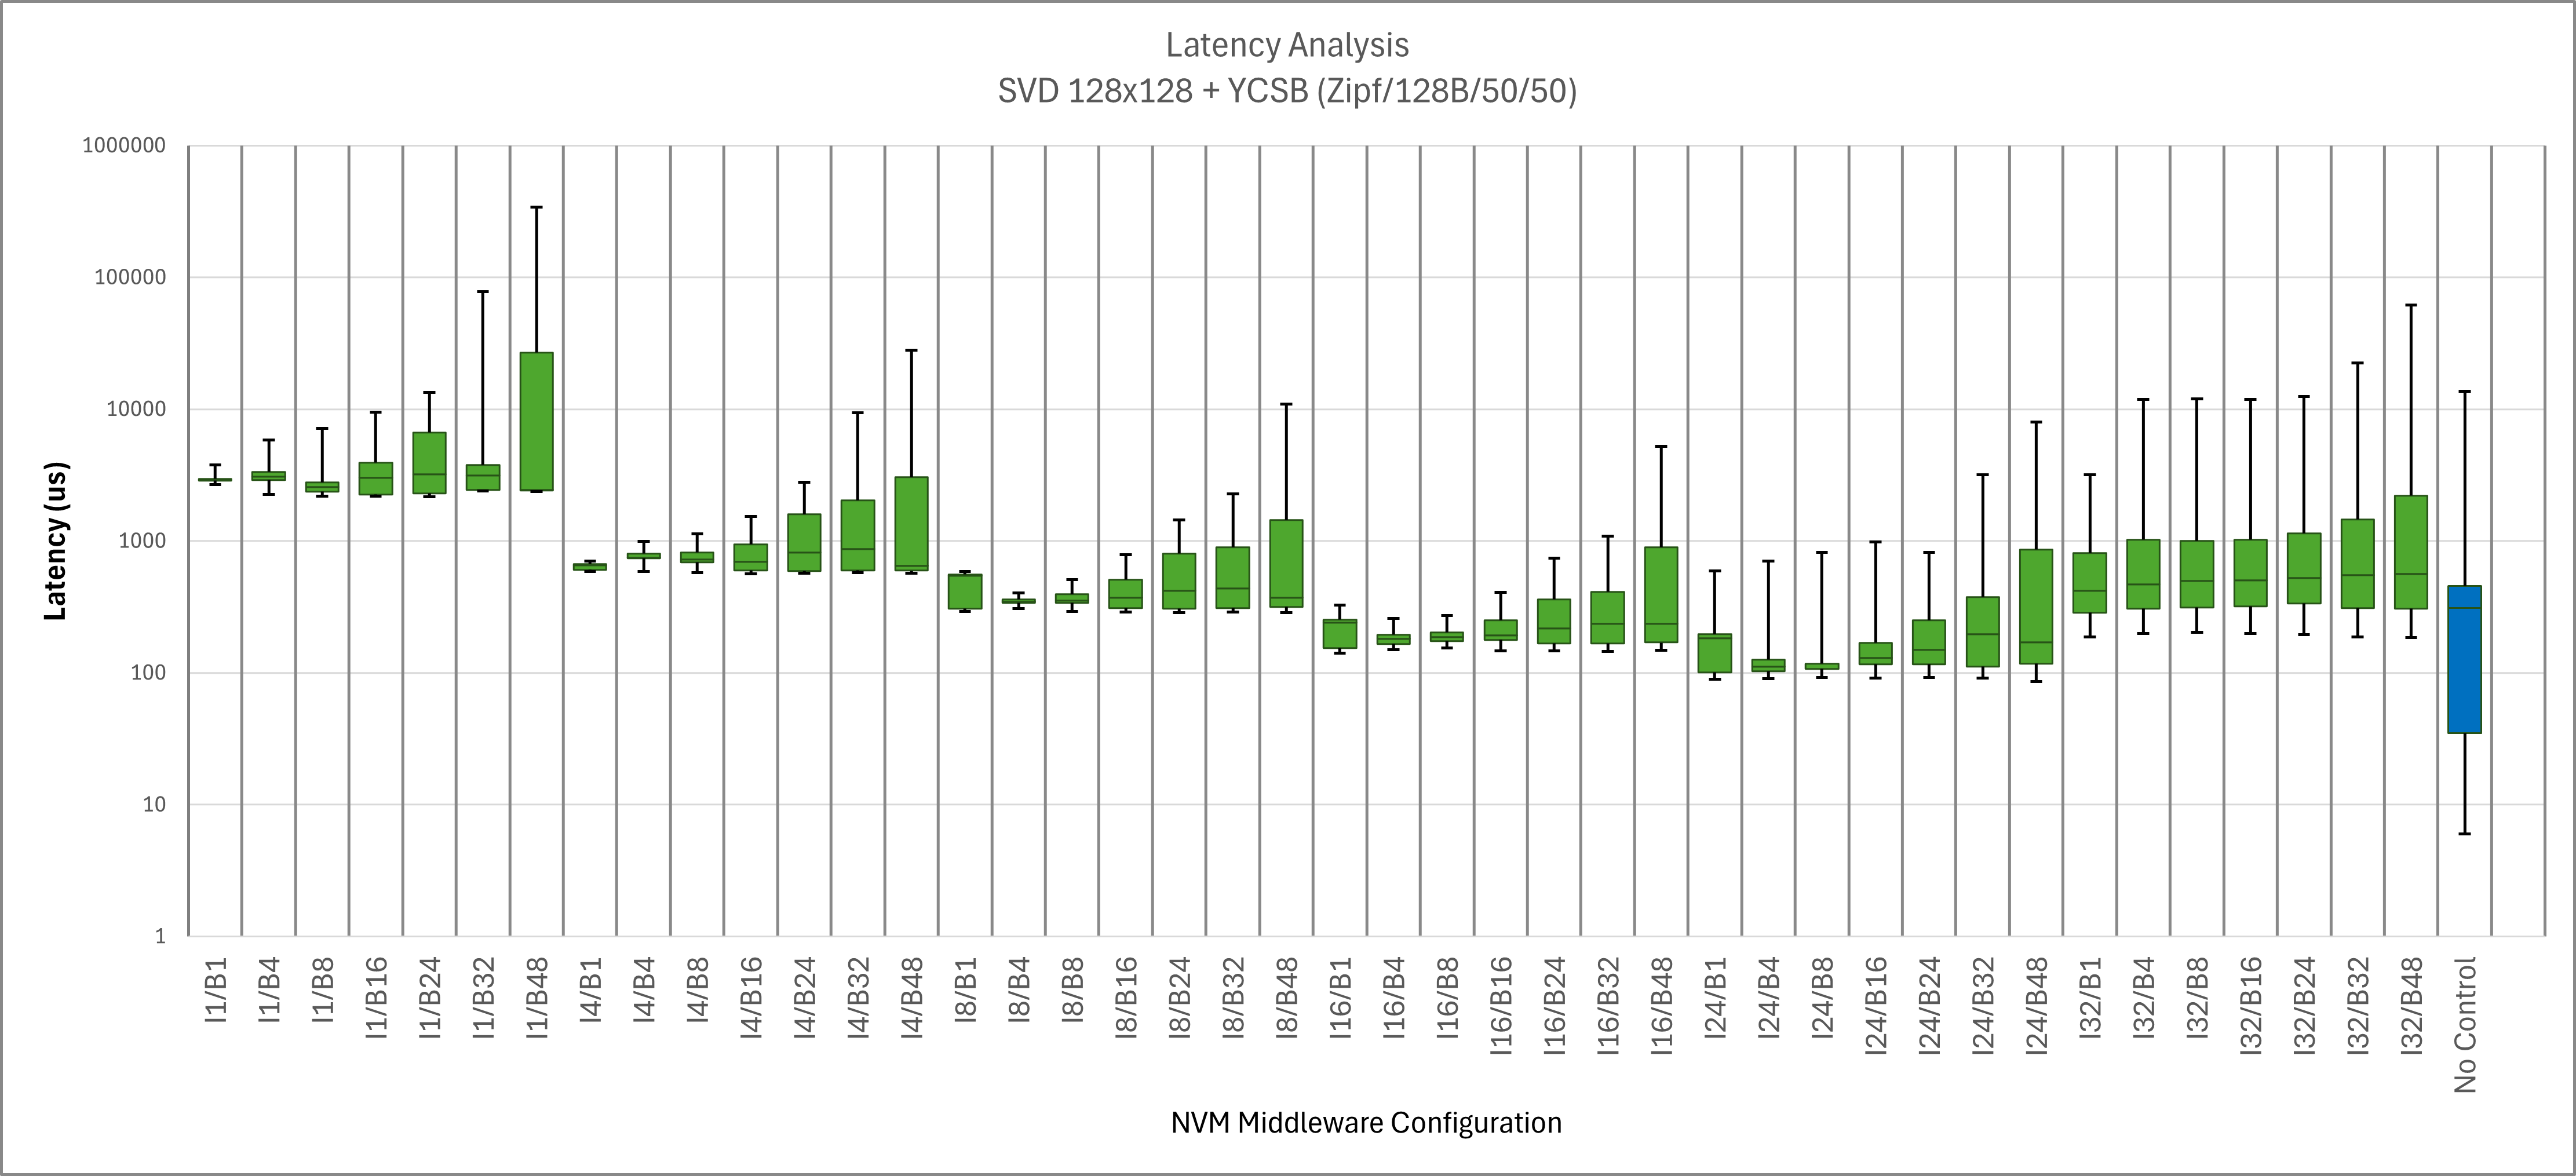
\includegraphics[width=\textwidth,height=\textheight,keepaspectratio,angle=0]{images/middleware-latency.png}
  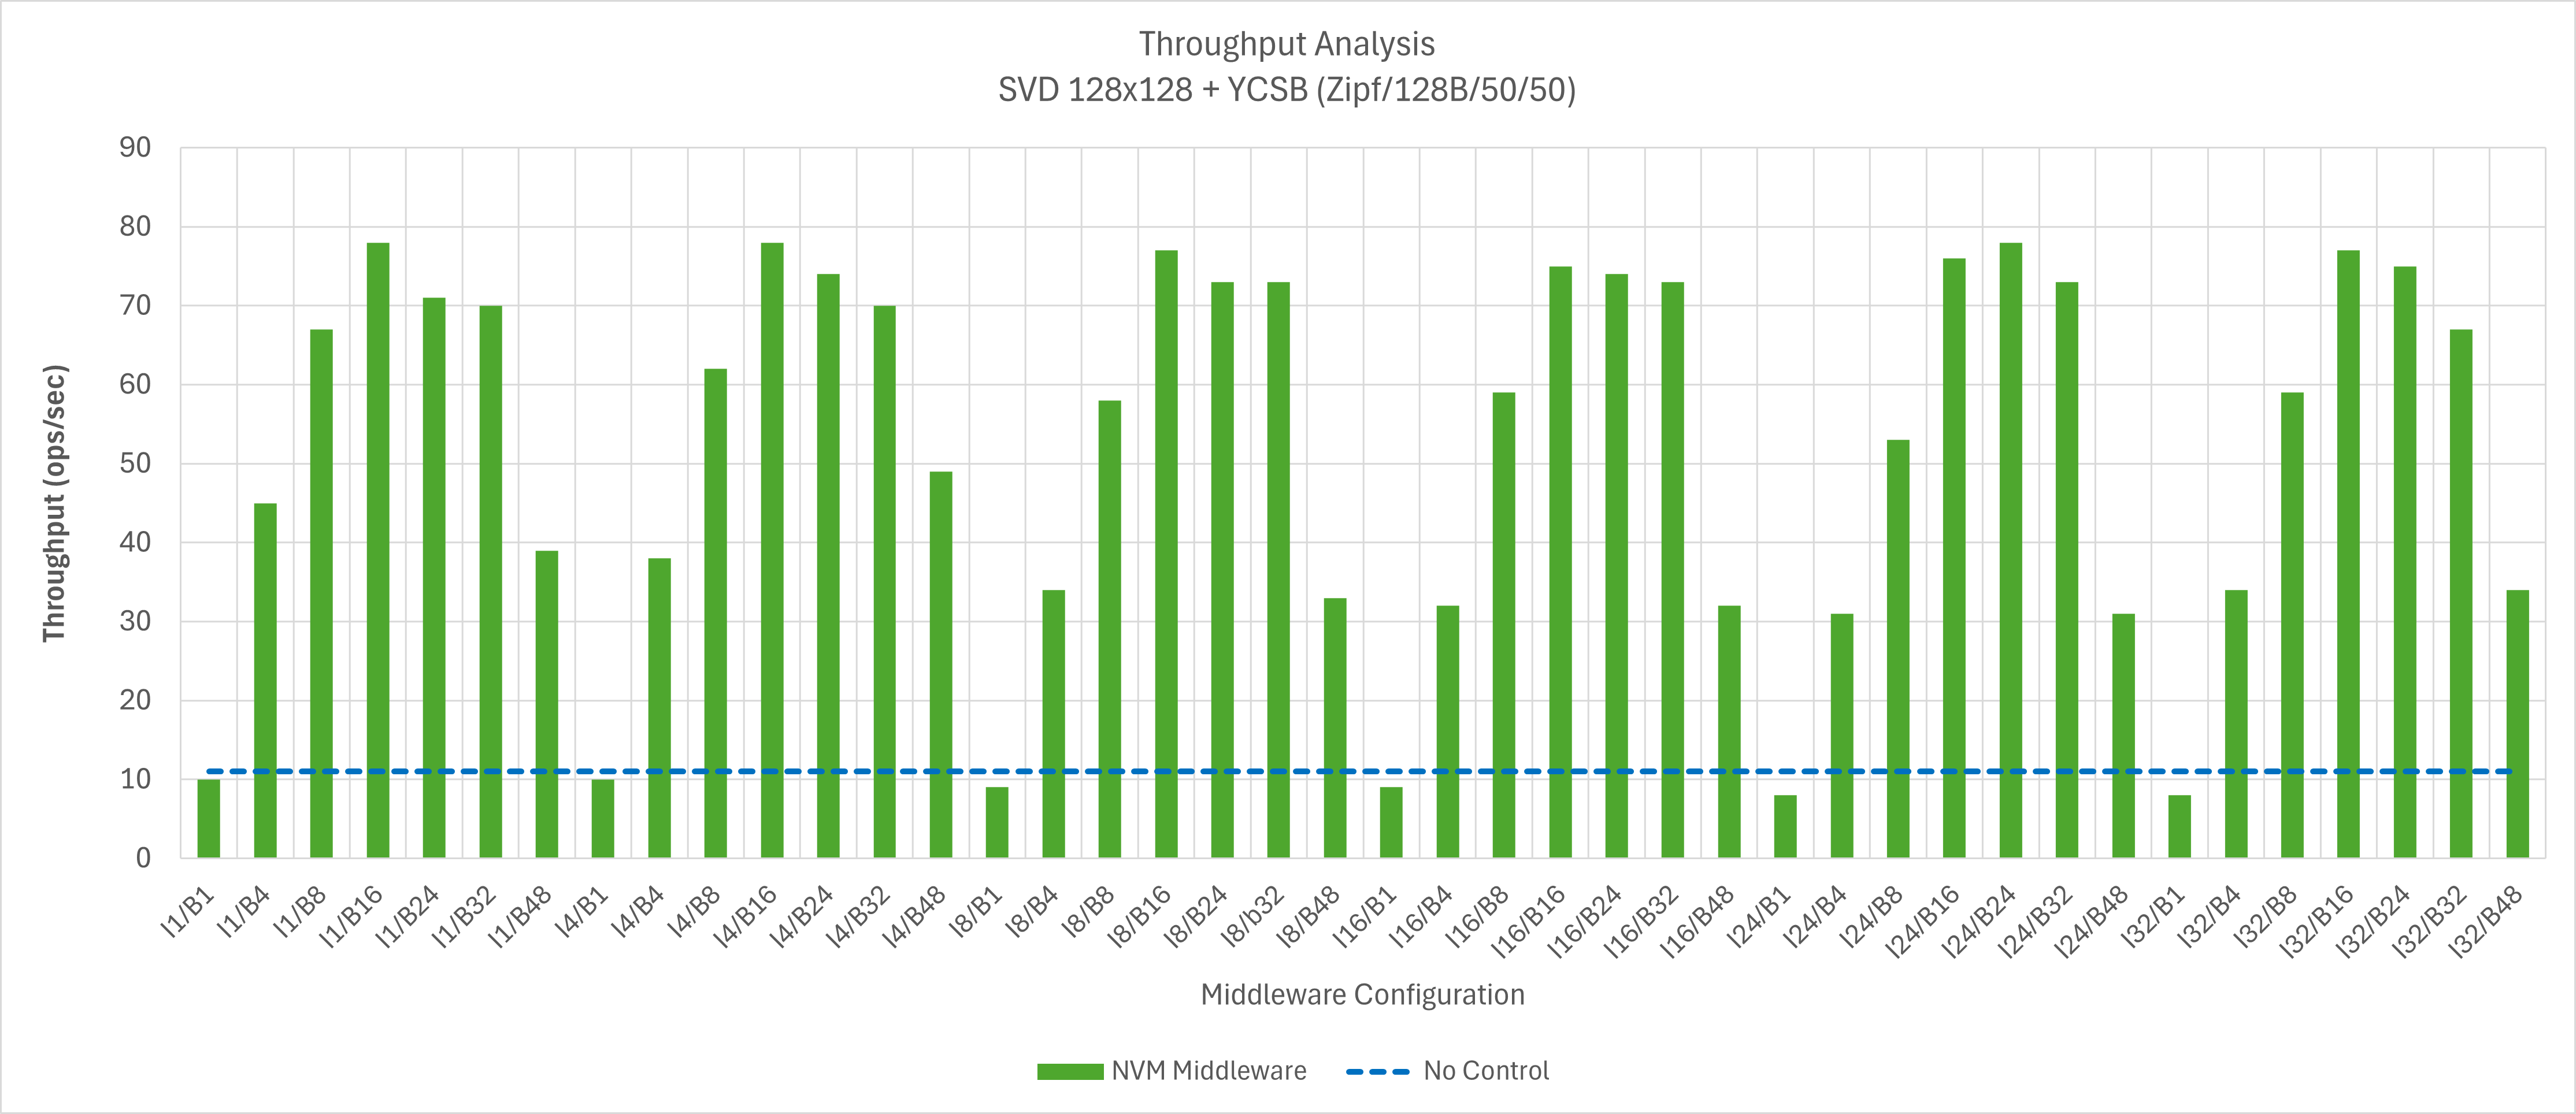
\includegraphics[width=\textwidth,height=\textheight,keepaspectratio,angle=0]{images/middleware-tp.png}
  \caption{Middleware Evaluation}
  \label{fig:middleware_eval}
\end{figure}

Our observations reveal that in most scenarios, both workloads derive substantial benefits from the concurrency control implemented by the NVM Middleware. Relative to the baseline, the NVM Middleware demonstrates the potential to enhance the 99th latency and throughput by up to 98\% and 86\%, respectively. Notably, the figure illustrates that the performance of applications is generally improved across most thread combinations. However, improper configuration of threads within the NVM Middleware, either too few or too many, leads to performance degradation surpassing that of the baseline. This underscores the importance for operators to meticulously select the optimal combination of threads, as an incorrect choice can yield inferior results compared to operating without any concurrency control.

A significant query stemming from these findings pertains to how an operator can determine the optimal thread combination. We observe that combining 16 interactive threads with fewer than 8 batch threads yields superior latency but fails to achieve peak throughput performance. Conversely, any combination with more than 16 batchs threads achieves peak throughput but incurs elevated access latencies. To address this dilemma, the ideal approach involves selecting the combination of interactive and batch threads that satisfies both latency and throughput SLA metrics, a topic further elaborated upon in the subsequent section.

\section{Q-Learning in Action}

\subsection*{Training the RL agent}

\subsection*{Evaluation on long-running test}
